%======================================================================
\section{Track ROB --- Robotics and drone kits}\label{sec:rob}
%======================================================================

These epics turn the general tracks into BruceWorx's own product domain: the Leonardo robot, servo arms
and quadcopters. Each one builds on a general epic, so nothing here forks the core design.

\begin{epic}{ROB-01}{COTS library \& insert}{M1}{\stTodo}{FCB-P2-09/10, P2R-01..04}
A COTS library folder with STEP models or datasheet envelopes plus per-part metadata: mass, CG offset,
mount pattern, category, supplier P/N, and for motors, kv and maximum thrust. The first set: NEMA17, 2207/2306
brushless motors, SG90/MG996R servos, 4-in-1 ESCs (30.5/20\,mm), 5'' props (disk envelope), and 608/6800
bearings (parametric). The insert command has a category picker and places \textbf{mounting LCSs}, so
\eref{ASM-03} quick joints and \eref{ASM-09} fasteners work immediately. COTS items get COTS P/Ns in PDM.
\emph{Acceptance:} a NEMA17 and a 2207 motor are inserted and jointed by their mounting LCS.
\end{epic}

\begin{epic}{ROB-02}{Frame \& arm templates}{M3}{\stTodo}{FCB-P2R-05/06}
A parametric quad X-frame (wheelbase, arm width, motor mount pattern) and a servo link/bracket (link length,
servo size), built as \textbf{configurations} (\eref{MOD-03}) rather than separate spreadsheets.
\emph{Acceptance:} the template regenerates cleanly for three wheelbases.
\end{epic}

\begin{epic}{ROB-03}{Mass, CG \& inertia report}{M1}{\stTodo}{FCB-P2R-07}
Per-part mass from density or a COTS override; totals, CG and the inertia tensor; CSV export and a 3D CG
marker. It builds on \eref{MOD-11}.
\emph{Acceptance:} the X-frame example in Figure~\ref{fig:cg}: 388.1\,g, CG at $(2.45, 0, -2.73)$\,mm.
\end{epic}

\begin{figure}[ht]
\centering
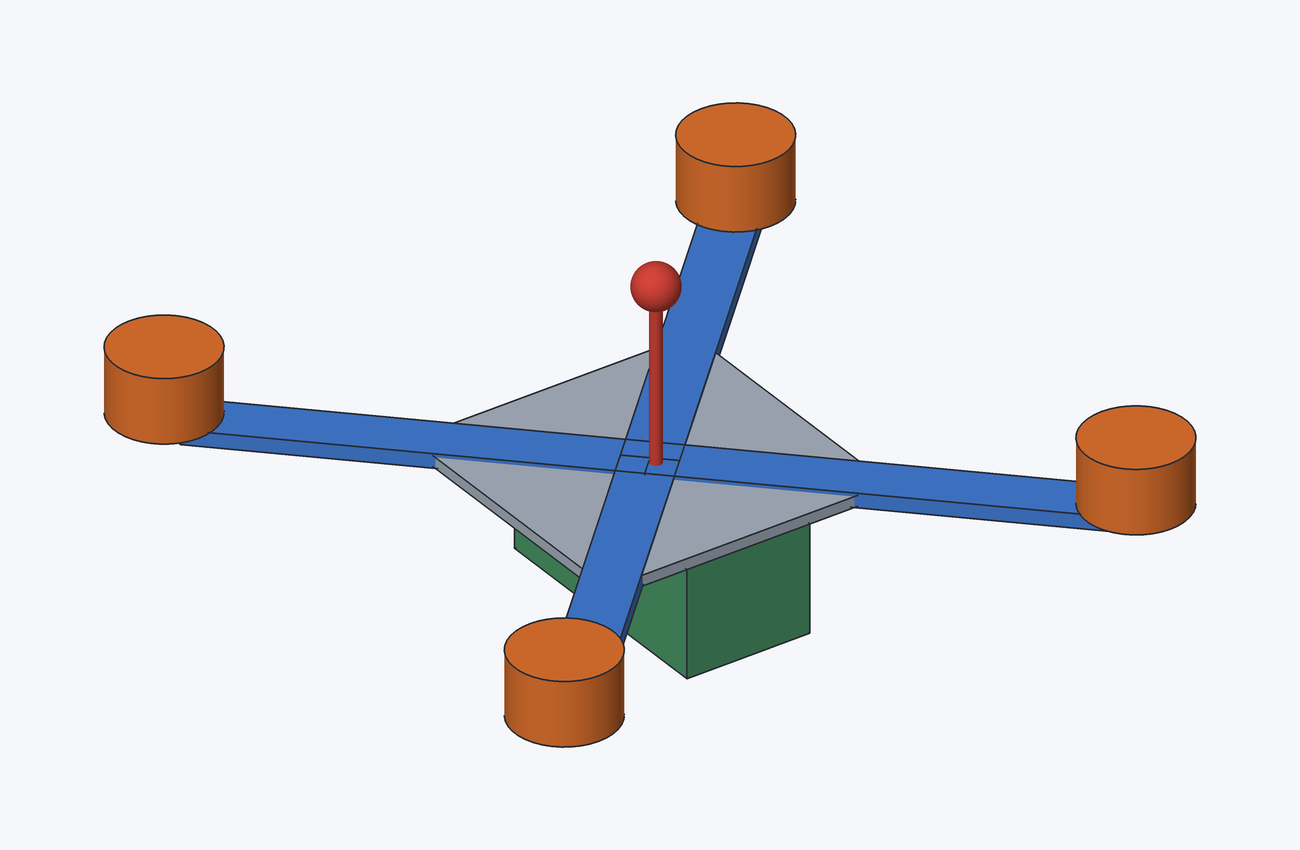
\includegraphics[width=0.55\linewidth]{fig/mass_cg.png}
\caption{Quad X-frame: carbon plate and arms from density (1.6\,g/cm$^3$), four 32\,g motors and a 190\,g
battery as COTS overrides. The battery is mounted 5\,mm forward, which puts the CG (red plumb line and
marker) at $x=2.45$\,mm. That is exactly what the balance check in \eref{ROB-04} must flag.
Computed in headless FreeCAD.}
\label{fig:cg}
\end{figure}

\begin{epic}{ROB-04}{Drone balance \& thrust-to-weight}{M3}{\stTodo}{FCB-P2R-08}
Compare the CG with the centroid of the motor axes, and report thrust-to-weight
$T/W=\sum_i T_{\max,i}/(m g)$ from COTS data. Warn when the horizontal CG offset exceeds a fraction of the
arm length, or $T/W<2$.
\emph{Acceptance:} the check flags the offset battery in Figure~\ref{fig:cg}.
\end{epic}

\begin{epic}{ROB-05}{Kinematic chains \& joint drive}{M5}{\stTodo}{FCB-P2A-09/10}
Build a link chain from revolute joints, show a joint table, read out end-effector forward kinematics, drive
the chain from the table through the stock Simulation (servo-sweep presets), and export video.
\emph{Acceptance:} the 2-DOF arm's FK matches a hand calculation.
\end{epic}

\paragraph{Theory: forward kinematics.} Each joint $i$ contributes a homogeneous transform
$T_i(\theta_i)=\begin{pmatrix}R(\mathbf a_i,\theta_i)&\mathbf p_i-R(\mathbf a_i,\theta_i)\mathbf p_i\\
\mathbf 0^{\!\top}&1\end{pmatrix}$, a rotation about its axis through $\mathbf p_i$ in the reference pose.
The end-effector pose is the product
\[
  T_{\text{ee}}(\boldsymbol\theta)=T_1(\theta_1)\,T_2(\theta_2)\cdots T_n(\theta_n)\,T_{\text{ee}}(\mathbf 0),
\]
the product-of-exponentials form, which needs no Denavit--Hartenberg frames and can be read directly from the
assembly's joints. For the planar 2-DOF arm, this reduces to
$x=\ell_1\cos\theta_1+\ell_2\cos(\theta_1+\theta_2)$ and $y=\ell_1\sin\theta_1+\ell_2\sin(\theta_1+\theta_2)$,
the acceptance check.

%======================================================================
\section{Track ECD --- ECAD bridge (KiCad)}\label{sec:ecd}
%======================================================================

\begin{epic}{ECD-01}{ECAD intake \& adopt-vs-build}{M1}{\stTodo}{FCB-P2E-01..04}
Requirements intake from the ECAD owner (KiCad version, outline and keep-outs, direction of placement sync,
STEP needs, sample board). Evaluate the KiCad StepUp add-on on current FreeCAD with a KiCad 9 board,
including its AGPL licence and maintenance. Then a decision memo: adopt StepUp unmodified, or build a bridge on
\code{kicad-cli} and the KiCad 9 IPC API. The Ops sample data shows this gate as done, but the result isn't
recorded (open question).
\end{epic}

\begin{epic}{ECD-02}{Board STEP into assembly}{M3}{\stTodo}{FCB-P2E-05}
Export with \code{kicad-cli pcb export step}, and insert into the assembly with an LCS at the board origin, so
the board joints like any component.
\end{epic}

\begin{epic}{ECD-03}{Board outline round-trip}{M3}{\stTodo}{FCB-P2E-06, P2E-09}
Pull \code{Edge.Cuts} into a Sketcher sketch and push edits back to \code{.kicad\_pcb}.
\emph{Acceptance:} the round-trip outline delta is below 0.01\,mm on the sample board.
\end{epic}

\begin{epic}{ECD-04}{Placement sync \& enclosure fit}{M3}{\stTodo}{FCB-P2E-07/08}
Push connector and mounting-hole positions from MCAD to ECAD and back. Check board against housing with the
interference command (\eref{ASM-06}).
\emph{Acceptance:} the fit check flags a connector moved into a wall.
\end{epic}

%======================================================================
\section{Track WIR --- Wire routing}\label{sec:wir}
%======================================================================

Servo arms, quad power leads and board-to-ESC runs need a wire that can be seen, measured and moved with
the joint. Fusion~360 has no harness product. This track is SolidWorks electrical-routing parity plus that
robotics need. It sits on M3 and M5, after joints exist (\eref{ASM-03}), and it stays off the M1 path that
models \code{LE-02001}.

The tube is ordinary FreeCAD. \code{Part.Wire.makePipeShell} sweeps a circle along a centerline, and
Draft's \code{filletWire} rounds every corner of a polyline to an exact radius. The centerline is that
polyline: a straight lead-out along the port's local $+Z$, then the clips, with each corner filleted.
The fillet radius is the minimum bend radius, and the centerline length is the cut length. Fillets hold
that minimum exactly, which a free B-spline cannot. BIM pipes are the same sweep at building scale and are
tied to IFC; they do not follow assembly links. The wire is its own \code{Part::FeaturePython}.

A port is an \code{App::LocalCoordinateSystem}, the same kind of datum as the mounting LCS in
\eref{ROB-01}. End placements come from \code{UtilsAssembly.getGlobalPlacement}, which already resolves a
link chain through \code{getPlacementOf}. A datum stays put when the model is edited; a face pick does not.
When \eref{WIR-02} starts, the add-on lives at \file{package/bruceworx/mods/WireRouting/}, installed the
same way as the History Timeline. Python only, no C++.

Following a joint is the part that takes care. The wire lives in the assembly, both ends are ports on
links, and a recompute after the solver moves a link rebuilds the centerline. Bundles are a small graph:
several wires share a sleeve, then break out. Clip-graph routing is a shortest path through clips the user
already placed, keeping a segment only when its fillet succeeds. Two commercial features stay off this
track: free-space auto-route through an obstacle mesh, and a flattened nailboard drawing. A fillet that
cannot be built is the bend-radius check. Clearance of the finished solid can later reuse
\eref{ASM-06}.

\eref{WIR-01} is a short adopt-versus-build spike, the same shape as \eref{ECD-01}. Try the community
Cables workbench on an assembly with two moving links, then write the decision down. Those add-ons route
inside one document. The spike is there so a workbench that cannot follow an \code{Assembly} joint is not
vendored. The expected result is to build.

\begin{epic}{WIR-01}{Adopt versus build}{M3}{\stTodo}{(new)}
Try the community Cables workbench on an assembly with two moving links. Record the decision: adopt it
unmodified, or build the Python add-on described above.
\emph{Acceptance:} the decision memo is written.
\end{epic}

\begin{epic}{WIR-02}{Port and wire}{M3}{\stTodo}{(new)}
A port datum, a straight lead-out along local $+Z$, \code{filletWire} at the minimum bend radius, a circle
swept with \code{makePipeShell}, and a read-only length.
\emph{Acceptance:} a three-corner wire matches the analytic line-plus-arc length within 0.01\,mm. A corner
tighter than the radius fails the check and produces no solid.
\end{epic}

\begin{epic}{WIR-03}{Assembly follow}{M3}{\stTodo}{(new)}
The wire lives in the assembly. Both ends are ports on links, and a recompute after the solver moves a
link rebuilds the centerline. Depends on \eref{WIR-02} and \eref{ASM-03}.
\emph{Acceptance:} dragging a revolute joint updates the length, and both ends stay on their ports.
\end{epic}

\begin{epic}{WIR-04}{From-to cut list}{M3}{\stTodo}{(new)}
Gauge, color, from, to and length for each wire. The assembly BOM (\eref{ASM-04}) carries the same rows.
\emph{Acceptance:} the cut list matches the wire lengths, and the BOM carries the rows.
\end{epic}

\begin{epic}{WIR-05}{Clips and bundles}{M5}{\stTodo}{(new)}
Clips are waypoints. A bundle is a shared sleeve with a breakout: several wires share a middle segment,
then split to their own ports. Depends on \eref{WIR-03}.
\emph{Acceptance:} two wires share one middle segment and split to two ports; the sleeve length is that
segment.
\end{epic}

\begin{epic}{WIR-06}{Route on the clip graph}{M5}{\stTodo}{(new)}
A from-to list becomes a shortest feasible path through clips the user placed. A segment is feasible when
its fillet succeeds. Board pins become ports only after \eref{ECD-04}; this epic does not wait on that.
\emph{Acceptance:} a three-clip fixture picks the shorter feasible path and reports its length.
\end{epic}
